% chapter 2 : tex-based documents
\chapter{Einf\"{u}hrung zu den \LaTeX-Dokumenten}

Bevor die wichtigsten {\tt .tex}-files besprochen werden, möchten wir noch auf
einige grundlegende Aspekte hinweisen:

\begin{itemize}
  \item Es wird ein gewisses Grundwissen in \LaTeX{} vorausgesetzt (man muss
    beileibe kein Experte sein, aber man sollte die wirklichen basics schon
    können). Ziel des vorliegenden Kapitels ist es, die Handhabung der 
    einzelnen {\tt .tex}-Dokumente des Vorlesungsbehelfs und der Übungsblätter
    zu skizzieren, nicht aber die Verwendung von \LaTeX{} von Grund auf zu 
    erklären. Sollte die Leserin bzw. der Leser noch keine Kenntnisse darin 
    haben, so  bietet sogar die TU Graz einige Tutorials dazu an 
    ({\tt \latextugraz}).\\
    Die Verwendung von \LaTeX{} ist, für die meisten Anwendung, ohnehin relativ
    einfach. Außerdem müssen viele Bachelor-/Masterprojekte und Masterarbeiten
    zwingend in \LaTeX{} verfasst werden. Zumal \LaTeX{}, sobald es beherrscht
    wird, sowieso jedwede herkömmliche Software zur Textverarbeitung schlägt,
    sollte das Erlernen nicht als Zeitverschwendung, sondern als Aneignung einer
    nützlichen Zusatzqualifikation angesehen werden.
  \item Der wichtigste Befehl beim Arbeiten mit dem Vorlesungsbehelf und
    den Übungsblättern ist {\bf copy-and-paste}. Um eine neue Übungsaufgabe zu
    Erstellen, kopiert man eine bestehende (die ähnlich aussieht), bennent sie
    entsprechend um, und passt sie adäquat an. Muss man eine neue Formel
    bzw. Gleichung schreiben, so sucht man die notwendigen Sonderzeichen in den
    bereits vorhandenen Formeln. Dies erspart nicht nur Arbeit, sondern stellt
    auch sicher, dass die Notation konsistent ist (z.B. dass das Symbol für 
    einen Vektor immer gleich aussieht). Es kommt eigentlich sehr selten vor, 
    dass gänzlich neue Konstrukte gebraucht werden, die nicht durch geschickten
    Einsatz von copy-and-paste erzeugt werden können.\\
    Ähnliches gilt beim Arbeiten mit {\tt Corel-Draw}: Muss ein neues Bild
    erstellt werden, so kopiert man sich am besten die Pfeile, Blöcke, Federn
    und sonstige Symbole aus bestehenden Bildern zusammen.
\end{itemize}

\section{Vorlesungsehelf (Formelsammlung)}

Beim Vorlesungsbehelf (bzw. der \glqq{}Formelsammlung\grqq{}) ist das file
\\\twrite{Vorlesungsbehelf\_Mechanik\_B3.tex} die Hauptdatei zur Kompilierung.
Es lädt die styles (z.B. die preambel) und die Inhalte (Deckblatt, Vorwort,
Kapitel, Anhänge).

In der folgenden Tabelle werden die Funktionsweise bzw. der Ablauf dieser
Datei anhand der wichtigsten Kommandos erklärt. Für das Verständnis ist es
ratsam, sich beim Durchlesen dieser Tabelle den \LaTeX-code nebenbei zu öffnen
und die einzelnen Punkte im echten Code zu identifizieren.

\newpage
\begin{center}
\large{\twrite{Vorlesungsbehelf\_Mechanik\_B3.tex}}
\end{center}

\begin{tabularx}{\textwidth}{l|X}%| disable odd look in emacs
  Kommando & Erklärung\\ \hline\hline
  % version
  \texcode{\textbackslash newcommand\{\textbackslash templateVersion\}}
  & Definiert die Versionsnummer.\\ \hline
  % preambel
  \texcode{\textbackslash input \{style/zs\_preambel\}}
  & Lädt die preambel für das zweiseitige Dokument. Für einseitigen Ausdruck:
    \texcode{es\_preambel}. Die preambel selbst sollte eigentlich nie editiert
    werden müssen.\\ \hline
  % macros
  \texcode{\textbackslash input \{style/macro\}}
  & Lädt die Makros. Die wichtigsten Makros sind:
    \begin{itemize}
      \item \texcode{\textbackslash wichtig}: Umschreibt den Text mit einem
        Rechteck.
      \item \texcode{\textbackslash wichtigm}: Analog zu 
        \texcode{\textbackslash wichtig}, zur Anwendung im \twrite{math mode}
        gedacht.
      \item \texcode{\textbackslash ten}: Das Symbol für Vektoren.
      \item \texcode{\textbackslash tens}: Das Symbol für Vektoren für
        griechische Buchstaben.
    \end{itemize}
    \\ \hline
  % isDraft
  \texcode{\textbackslash newcommand\{\textbackslash isDraft\}}
  & Eigentlich muss man den Entwurfszustand nicht als solche Kennzeichnen. Es
    sollte reichen diese Variable immer \texcode{false} zu setzen.\\ \hline
  % some variables
  einige weitere Variablen
  & Anhand der Kommentare kann man leicht erkennen, was welche Variable
    steuert.\\ \hline
  % begin
  \texcode{\textbackslash begin \{document\}}
  & Folgender Abschnitt wird in In \figref{fig:fsmain} dargestellt.\\\\
  % deckblatt
  \texcode{\textbackslash input \{content/0\_deckblatt\}}
  & Lädt das Deckblatt. Im Deckblatt scheinen folgende Dinge auf, die beim
    Wechsel von einem Studienjahr auf das nächste möglichweise editiert werden 
    müssen:
    \begin{itemize}
      \item Name des Dokuments (\glqq{}Vorlesungsbehelf\grqq{})
      \item Namen der Studienrichtungen (Bau, Verfahrenstechnik, Mathematik)
      \item akutelles Studienjahr
    \end{itemize}   
    \\\\
  % einleitung
  \texcode{\textbackslash input \{content/0\_einleitung\}}
  & Lädt die Einleitung. In der Einleitung scheint das Studienjahr auf, und muss
    somit beim Wechsel auf ein neues Studienjahr aktualisiert werden.\\\\
  % kapitel
  \texcode{\textbackslash input \{...\}} Kapitel 1-10 (11)
  & Einfügen der Kapitel 1-10 und des Anhanges (Kapitel 11). Im Ordner
    \twrite{content} existieren mehr {\tt .tex}-Kapitel als diese 11, jedoch 
    sind nur genau diese relevant (die anderen sind lediglich Überbleibsel von 
    früher).\\\\
  % end
  \texcode{\textbackslash end \{document\}}
  &
\end{tabularx}

\begin{figure}[htbp]
  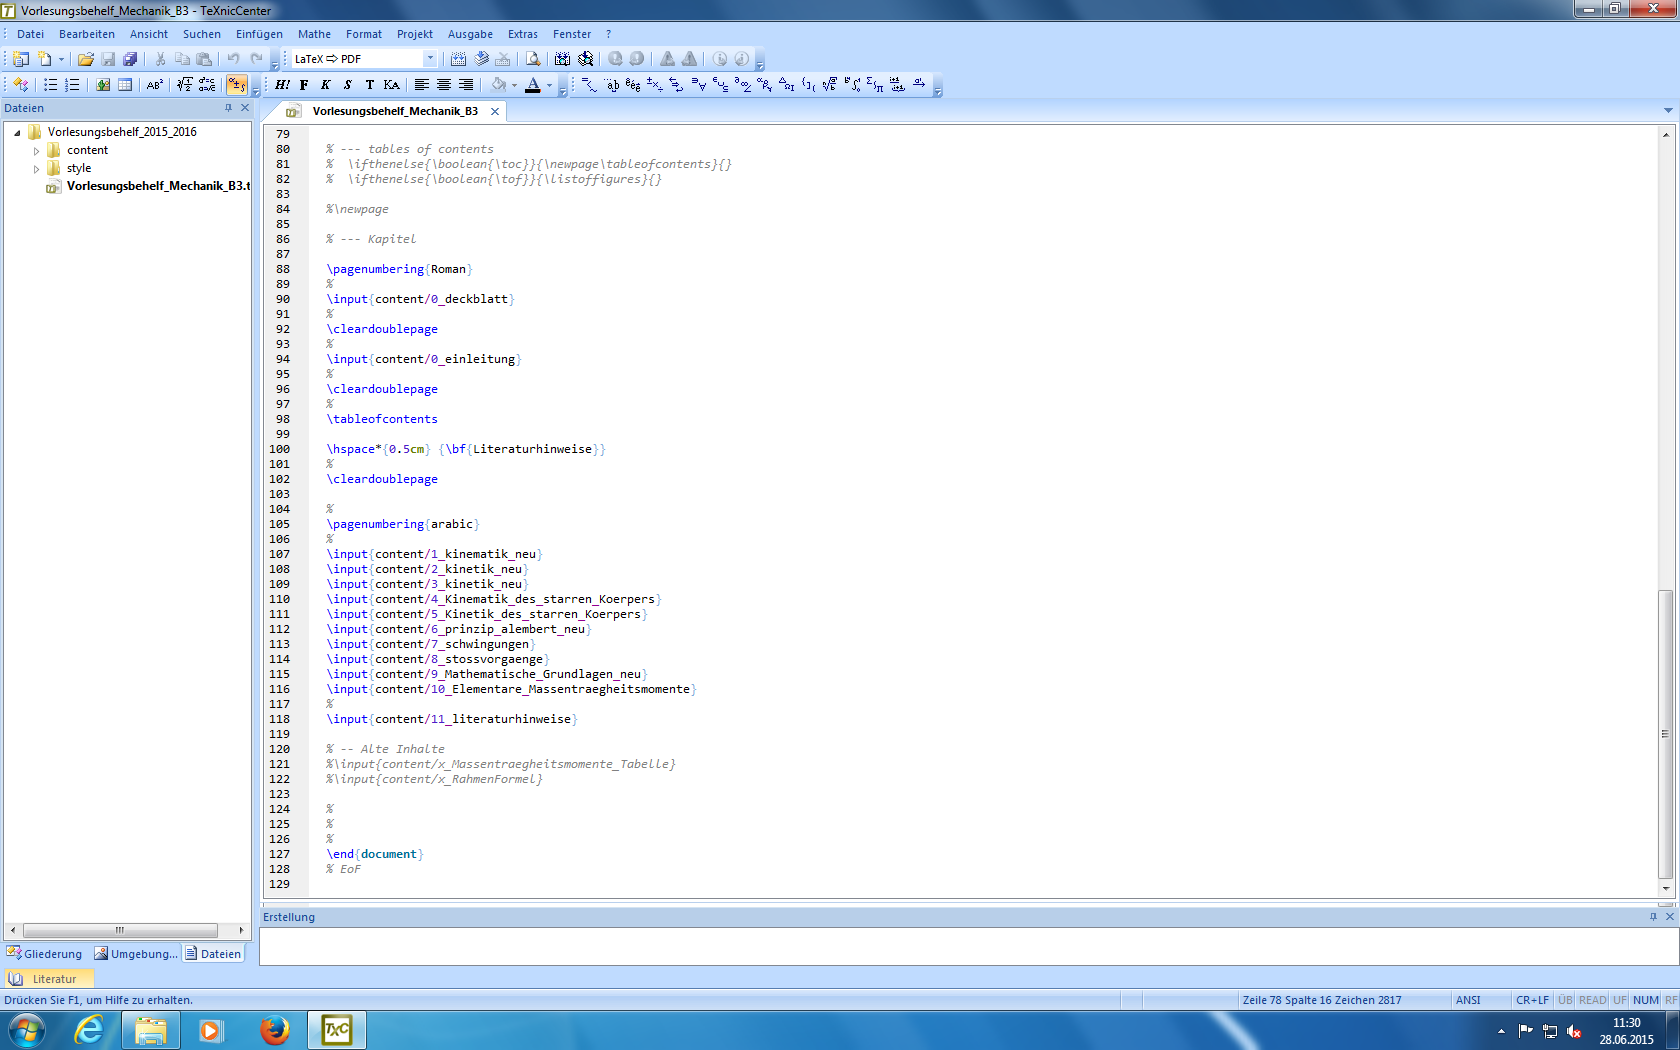
\includegraphics[width=\textwidth]{1_fsMain.png}
  \caption{Der eigentliche Kern von \twrite{Vorlesungsbehelf\_Mechanik\_B3.tex}.
    Oben werden Deckblatt und Einleitung geladen, während im unteren Block alle
    Kapitel eingefügt werden.}
  \label{fig:fsmain}
\end{figure}

\newpage
\section{\"{U}bungsbl\"{a}tter}

Wie bereits im ersten Kapitel erwähnt, werden alle drei übungsbezogenen 
Dokumente (Angaben, Durchgerechnete und Lösungen) aus dem file 
\twrite{Aufgaben.tex} erstellt. Es wird explizit darauf hingewiesen, dass die 
Funktionsweise bei den Übungsblättern ewas anders als bei der Formelsammlung 
ist.

Das Wichtigste zum Verständnis ist, dass in \twrite{Aufgaben.tex} die Variable
(bzw. eigentlich das Kommando) \texcode{\textbackslash myVar} mittels
\texcode{\textbackslash newcommand\{\textbackslash myVar\}\{X\}} definiert ist.
Je nachdem welcher Wert für \texcode{X} eingesetzt wird, wird ein anderes
Dokument kompiliert. Alle möglich Werte von \texcode{X} sind im \TeX-Code an 
dieser Stelle mit Kommentaren beschrieben, und in folgender Tabelle werden nur 
noch die wichtigsten Werte angeben.

\begin{tabularx}{\textwidth}{l|X}%| disable odd look in emacs
  Kommando  & Erzeugtes Dokument \\
  \hline
  \texcode{\textbackslash newcommand\{\textbackslash myVar\}\{1\}}
  & Angaben zu den Aufgaben für Mechanik B3 (Baumechanik 3), Dynamik VT\\
  \hline
  \texcode{\textbackslash newcommand\{\textbackslash myVar\}\{10\}}
  & Angaben zu den Aufgaben für Mechanik - Dynamik\\
  \hline
  \texcode{\textbackslash newcommand\{\textbackslash myVar\}\{3\}}
  & Lösungen (alle Studienrichtungen)\\
  \hline
  \texcode{\textbackslash newcommand\{\textbackslash myVar\}\{5\}}
  & Durchgerechnete Beispiele (alle Studienrichtungen)
\end{tabularx}

Die erzeugten Dokumente bei \texcode{X}=1 und \texcode{X}=10 weichen nur im 
Deckblatt voneinander ab (der Wert 10 ist hierbei als \glqq{}eins-null\grqq{} 
zu verstehen).

\newpage
\begin{center}
\large{\twrite{Aufgaben.tex}}
\end{center}

\begin{tabularx}{\textwidth}{l|X}%| disable odd look in emacs
  Kommando & Erklärung\\ \hline\hline
  % preambel
  \texcode{\textbackslash input \{Basisdaten/style/preambel\}}
  & Lädt die preambel. Im Gegensatz zur Formelsammlung gibt es keine
    Unterscheidung zwischen ein- und zweiseitigem Ausdruck. Es gilt hier auch,
    dass die preambel selbst eigentlich nie verändert werden sollte.\\ \hline
  % macros
  \texcode{\textbackslash input \{Basisdaten/style/macro\}}
  & Lädt die Makros. Praktisch ident zur Formelsammlung.
    \\ \hline
  % reference
  & Folgender Abschnitt wird in In \figref{fig:aufgabemain} dargestellt.\\
  % myVar
  \texcode{\textbackslash newcommand\{\textbackslash myVar\}\{X\}}
  & Anhand der Kommentare kann man ablesen, welche Werte \texcode{X}
    annehmen darf und was jeder Wert repräsentiert.\\\\
  % variable
  \texcode{\textbackslash input \{Basisdaten/style/variable\}}
  & Lädt das Dokument \twrite{variable.tex}. Dieses ist sozusagen der Pivot
    in der Erstellung des Dokuments und wird im Folgenden noch genauer
    besprochen.\\\\
  % begin
  \texcode{\textbackslash begin \{document\}}
  & \\
  % deckblatt
  \texcode{\textbackslash myDeckblatt}
  & Fügt das Deckblatt ein, welches in \twrite{variable.tex} definiert wird.  
    \\\\
  % inhalt
  \texcode{\textbackslash input \{content/0\_einleitung\}}
  & Fügt den Inhalt ein, welcher in \twrite{variable.tex} definiert wird.\\
  % end
  \texcode{\textbackslash end \{document\}}
  &
\end{tabularx}

\begin{figure}[htbp]
  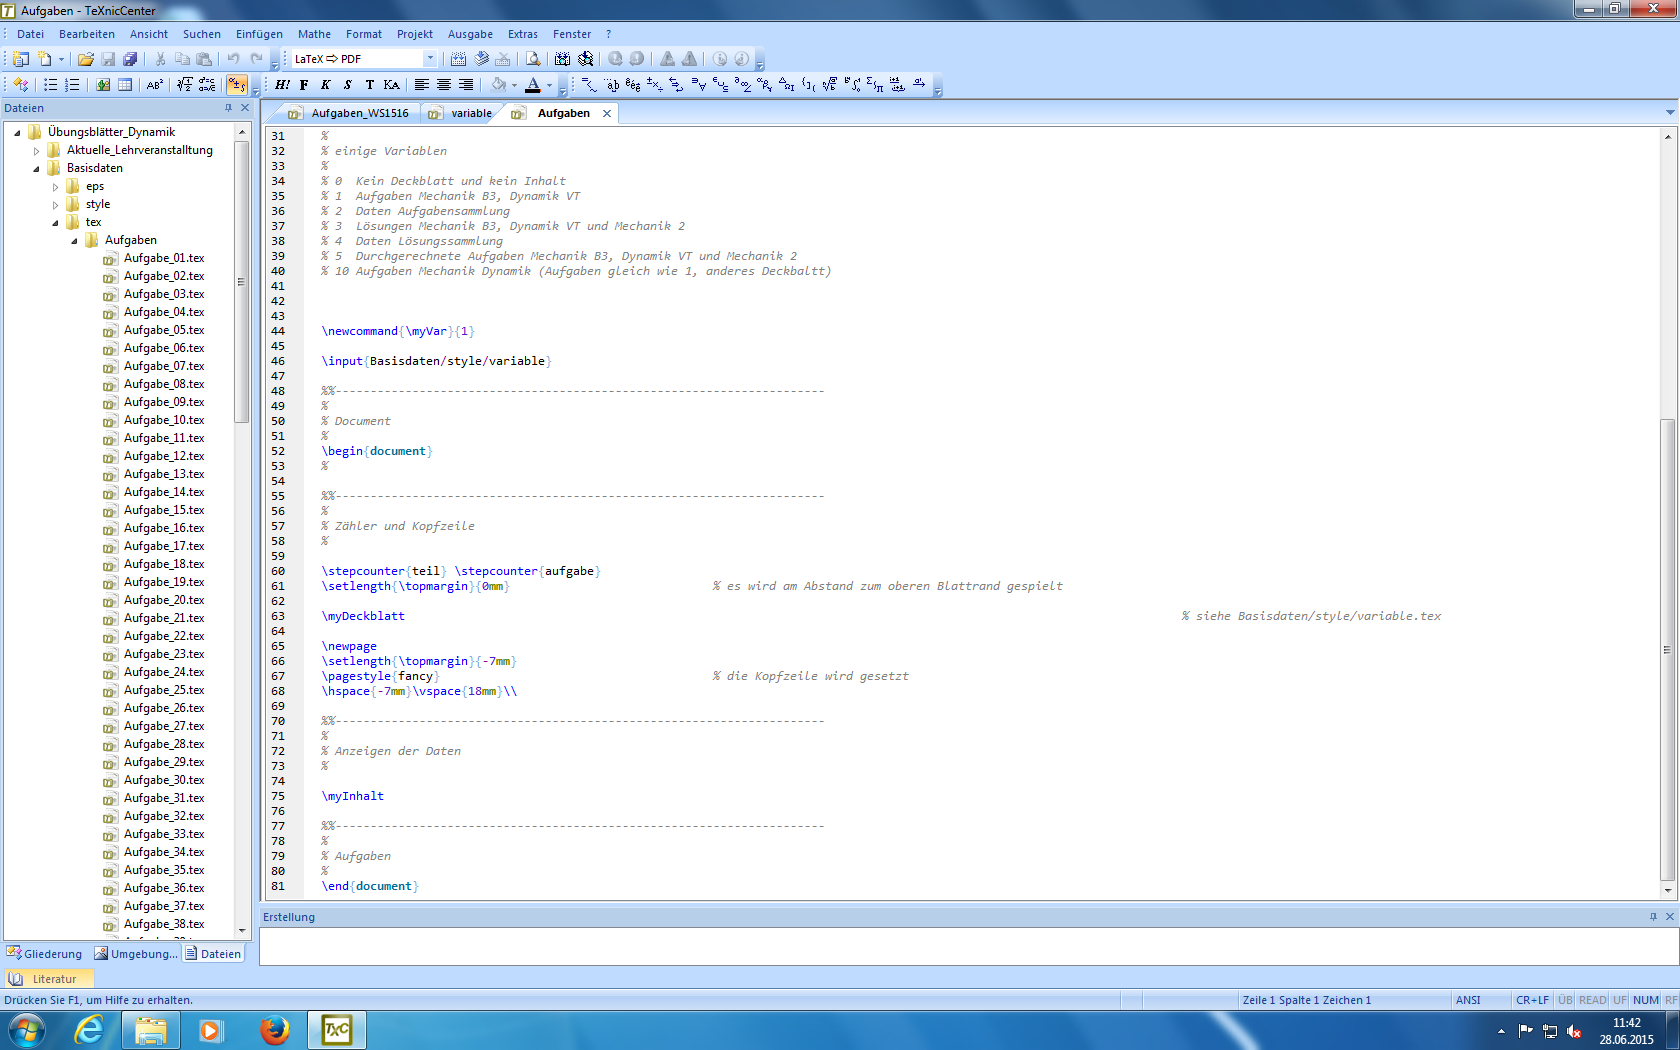
\includegraphics[width=\textwidth]{1_aufgabeMain.png}
  \caption{Der Hauptteil von \twrite{Aufgabe.tex}. Oben wird 
    \texcode{\textbackslash myVar} definiert, wobei die einzelnen Werte im
    Kommentar beschrieben werden. Darunter wird die \twrite{variable} inkludiert
    und weiter unten mit \texcode{\textbackslash myDeckblatt} und 
    \texcode{\textbackslash myInhalt} das eigentliche Dokument eingefügt.}
  \label{fig:aufgabemain}
\end{figure}


\subsection{Dokument \twrite{variable.tex}}

Dieses file ist der Dreh- und Angelpunkt bei den Übungsblättern. Es ist
grundsätzlich in zwei Blöcke gegliedert, die im Folgenden kurz erklärt werden.

\begin{itemize}
 \item {\bf 1. Block}: Im ersten Block werden sehr viele Variablen definitert. 
   Einige davon sind:
   \begin {itemize}
    \item aktuelles Studienjahr
    \item Namen der Studienrichtungen (Bau, Verfahrenstechnik, Mathematik)
    \item Termine (Übungsblattabgabe, Prüfung, Tutorien, \dots)
    \item die Nummern der für die Übungsblattabgabe relevanten Beispiele
   \end{itemize}
   Grundsätzlich kann man beim Durchlesen des \TeX-codes leicht erkennen, was
   welche Variable bedeutet. Beim Wechseln von ein Studienjahr auf das nächste
   sind die meisten Aktualisierungen in genau diesem Block vorzunehmen.
 \item {\bf 2. Block}: Der zweite Block ist in \figref{fig:variable} 
   dargestellt. Hier werden zunächst die Kursnamen (bzw. eigentlich die Namen
   der Dokumente) in Abhängigkeit von \texcode{\textbackslash myVar}
   festgelegt. Dazu wird die \LaTeX-Implementierung des 
   {\bf if-else}-conditionals \texcode{\textbackslash ifthenelse} verwendet.
   Darunter werden die Variablen \texcode{\textbackslash myDeckblatt} und
   \texcode{\textbackslash myInhalt} enstprechend definiert. Diese Variablen
   bestimmen im Endeffekt nur welches Deckblatt und welche Datei der Inhalte
   mittels \texcode{\textbackslash include} geladen werden sollen. Die 
   Deckblätter müssen selbst eigentlich nicht editiert werden, die 
   Dateien der Inhalte aber schon. Die relevanten Dateien werden im Folgenden 
   angeführt.
\end{itemize}

\begin{figure}[htbp]
  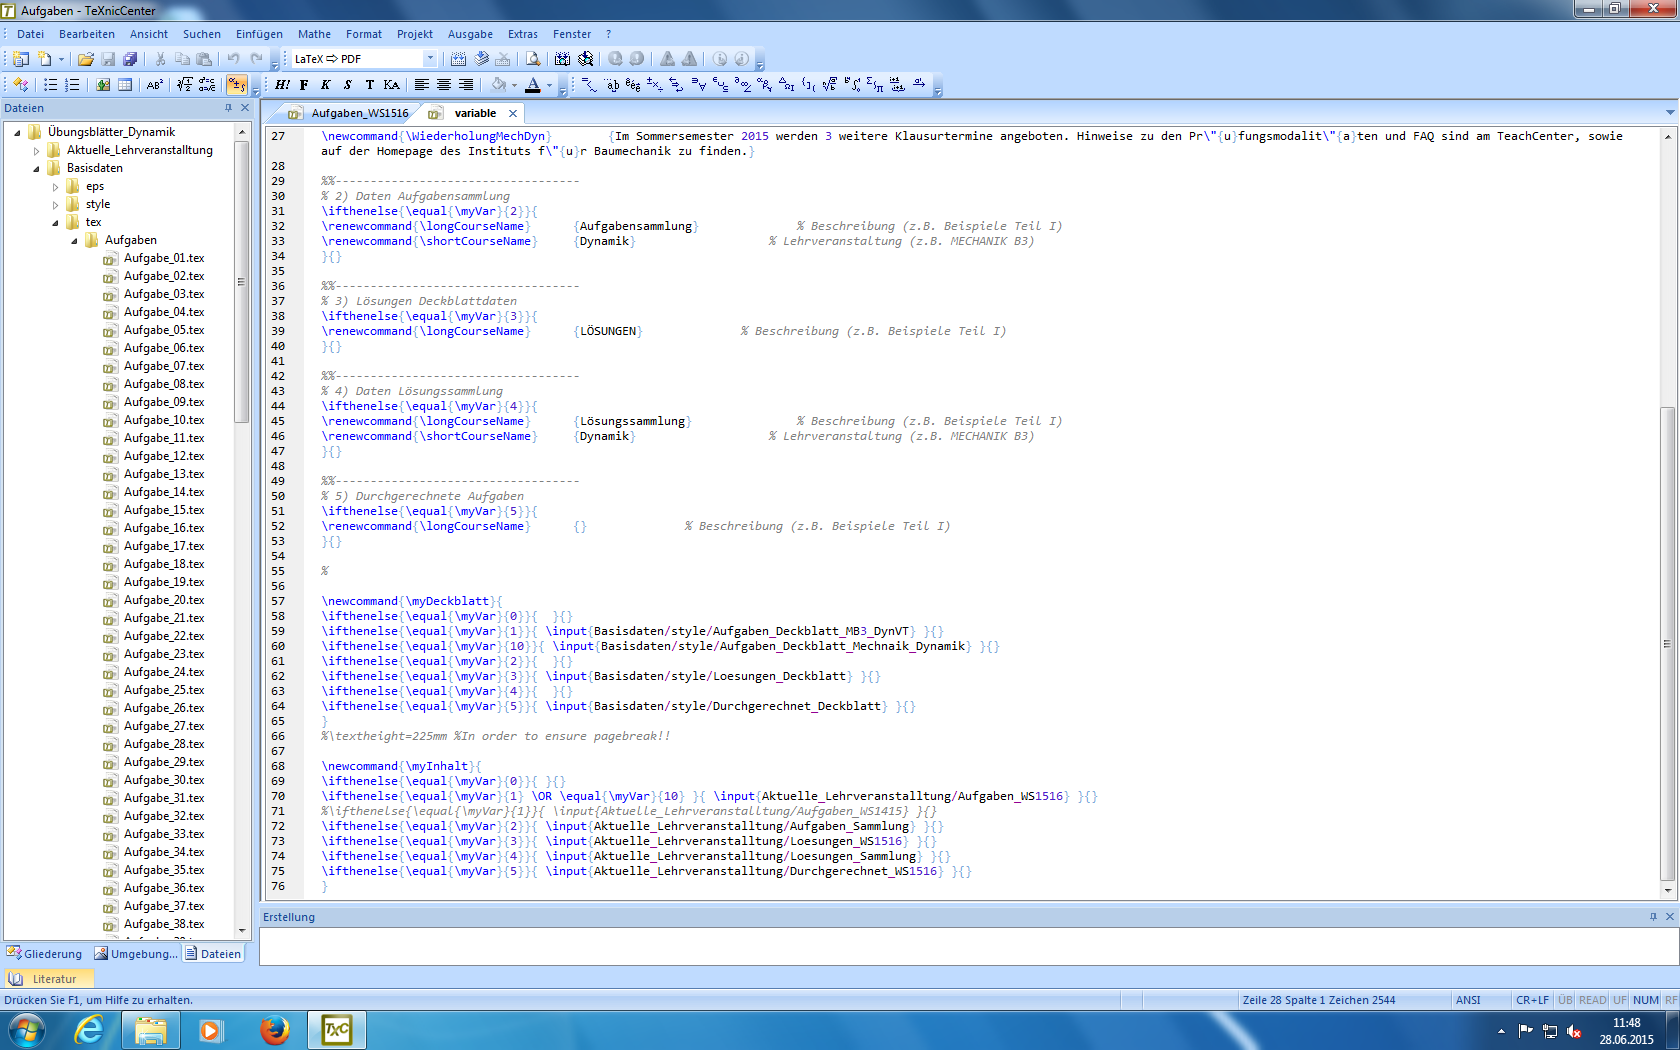
\includegraphics[width=\textwidth]{1_variable.png}
  \caption{Ausschnitt von \twrite{variable.tex}. Oben werden Variablen mit
    den Kursnamen definiert, und unten den Kommandos
    \texcode{\textbackslash myDeckblatt} und \texcode{\textbackslash myInhalt}
    in Abhängigkeit von \texcode{\textbackslash myVar} das richtige Dokument
    zugewiesen. Man kann hier leicht erkennen, dass für die Werte 1 und 10
    unterschiedliche Deckblätter, aber der selbe Inhalt geladen werden
    (man beachte das \texcode{OR} im \texcode{\textbackslash ifthenelse}). Die
    relevanten Inhalte werden in den Fällen 1 (bzw. 10), 3 und 5 geladen.}
  \label{fig:variable}
\end{figure}

\subsection{Dateien der Inhalte (zB. \twrite{Aufgaben\_WSyyzz.tex})}

Die relevanten Inhalte werden in den Fällen 1 (bzw. 10), 3 und 5 geladen.
Diese Dateien sind:

\begin {itemize}
 \item \twrite{Aufgaben\_WSyyzz.tex}
 \item \twrite{Loesungen\_WSyyzz.tex}
 \item \twrite{Durchgerechnet\_WSyyzz.tex}
\end{itemize}

Die meisten anderen Dokumente sind \glqq{}Sammlungen\grqq{}, d.h. es werden
einfach alle Beispiele, die es gibt, geladen. Allerdings werden diese Sammlungen
praktisch nie genutzt.

Die obigen drei Dateien der Inhalte sind alle im Endeffekt gleich aufgebaut. 
Deshalb betrachten wir im Folgenden nur noch die Datei 
\twrite{Aufgaben\_WSyyzz.tex}, da die beiden anderen konzeptuell ident sind.

In \figref{fig:aktaufgabe} ist ein Teil der Datei \twrite{Aufgaben\_WS1516.tex},
dargestellt. Hier werden alle {\tt .tex}-Dateien der Aufgaben 
(\twrite{Aufgabe\_xx.tex}) nacheinander in der vorgschriebenen Reihenfolge 
inkludiert. Hierbei ist Folgendes wichtig: Die \glqq{}interne\grqq{} Nummer 
eines Beispiels (\twrite{Aufgabe\_111.tex} hat die interne Nummer 111) 
hat nichts mit der Reihenfolge des Erscheinens im fertigen Dokument zu tun. 
Wird \twrite{Aufgabe\_111.tex} als drittes durch 
\texcode{\textbackslash include} geladen, so ist es natürlich auch das dritte 
Beispiel. Die korrekte fortlaufende Nummerierung der Beispiele wird durch einen
internen Zähler sichergestellt, der durch \texcode{\textbackslash stepcounter}
nach jedem \texcode{\textbackslash include} inkrementiert wird.

\begin{figure}[htbp]
  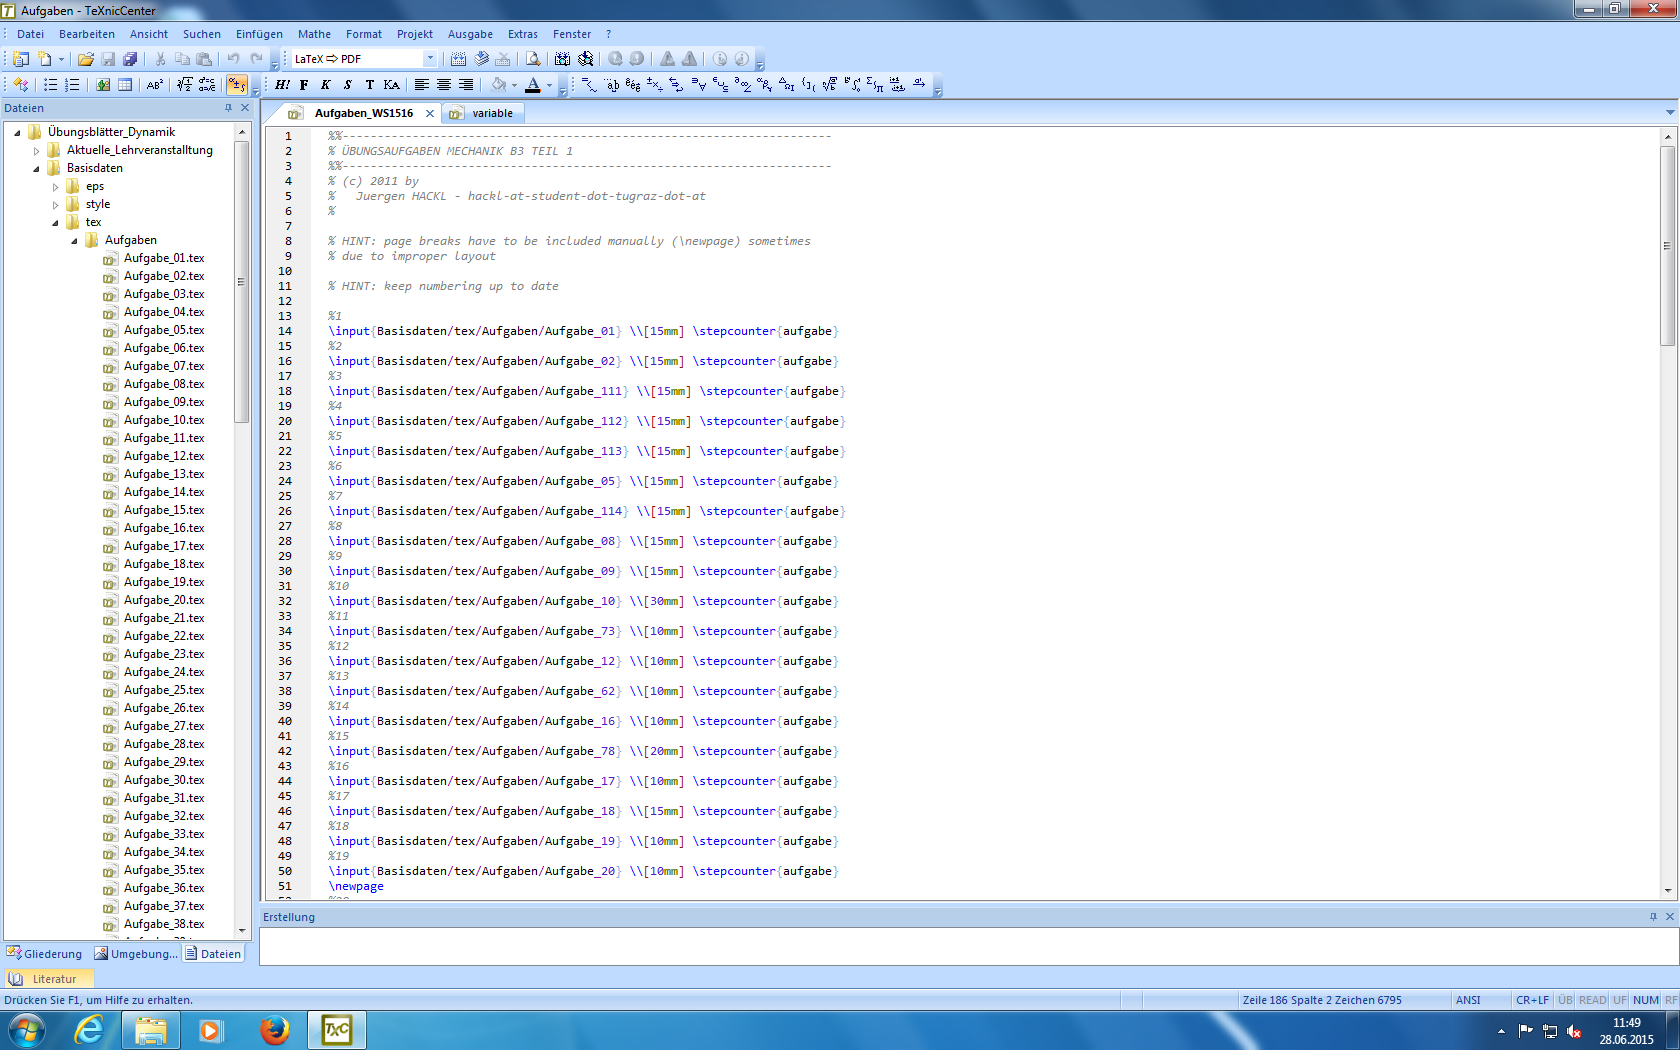
\includegraphics[width=\textwidth]{1_aktAufgabe.png}
  \caption{Ausschnitt von \twrite{Aufgaben\_WS1516.tex}. Die einzelnen
    Aufgaben werden nacheinander eingefügt. Man beachte, dass 
    \texcode{\textbackslash stepcounter} dafür zuständig ist, dass die Beispiele
    im fertigen Dokument richtig (fortlaufend) nummeriert sind.}
  \label{fig:aktaufgabe}
\end{figure}

\subsection{Datei eines Beispiels (z.B. \twrite{Aufgabe\_xx.tex}) }

Hier wird noch exemplarisch die Datei zu einem Beispiel
(\twrite{Aufgabe\_xx.tex}) diskutiert.

In \figref{fig:aufgabe01} wird die Datei \twrite{Aufgabe\_01.tex} dargestellt.
Zuerst wird der Text zur Aufgabe in eine \texcode{\textbackslash minipage}
geschrieben. Es ist darauf zu achten, dass es zwei grundsätzlich verschiedene 
Layouts gibt:

\begin {enumerate}
 \item Der Text (mit den Fragen) geht über die halbe Seitenbreite und die 
   Skizze ist daneben. Hier sind zwei gleich hohe minipages nebeneinander
   angeordnet.
 \item Der Text geht über die gesamte Seitenbreite und darunter sind die Fragen
   neben der Skizze. Hier ist eine kurze minipage über die gesamte Breite und
   darunter zwei gleich hohe minipages nebeneinander angeordnet
   (\twrite{Aufgabe\_01.tex} hat genau dieses Layout).
\end{enumerate}

Nach dem Text wird das Bild eingefügt. Die Beschriftung der Bilder erfolgt 
direkt in \LaTeX{} in der 
\texcode{\textbackslash overpic}-Umgebung mit dem Befehl
\texcode{\textbackslash put(x,y)\{...\}}, wobei \texcode{x} und \texcode{y}
die Koordinaten darstellen. Um das Beschriften leichter zu gestalten, kann man
sich ein Koordinatennetz anzeigen lassen, indem man den Befehl 
\texcode{grid,tics=n} bei der Bildbreite dazuschreibt.
Um im unteren Beispiel ein Koordinatennetz zu zeichnen, muss die 25. Zeile wie
folgt umgeschrieben werden:
\begin{center}
\texcode{\textbackslash begin\{overpic\}[width=6.5cm,grid,tics=5]\{Grafik\_1\}}
\end{center}
Der Abstand der Netzlinien wurde hier mit 5 gewählt, in manchen Fällen ist aber
10 besser geeignet.

Muss man ein neues Beispiel erstellen, so is es ratsam, ein bestehendes (mit dem
richtigen Layout) zu kopieren und nur den Text, die Fragen und das Bild 
zu ändern.

\begin{figure}[htbp]
  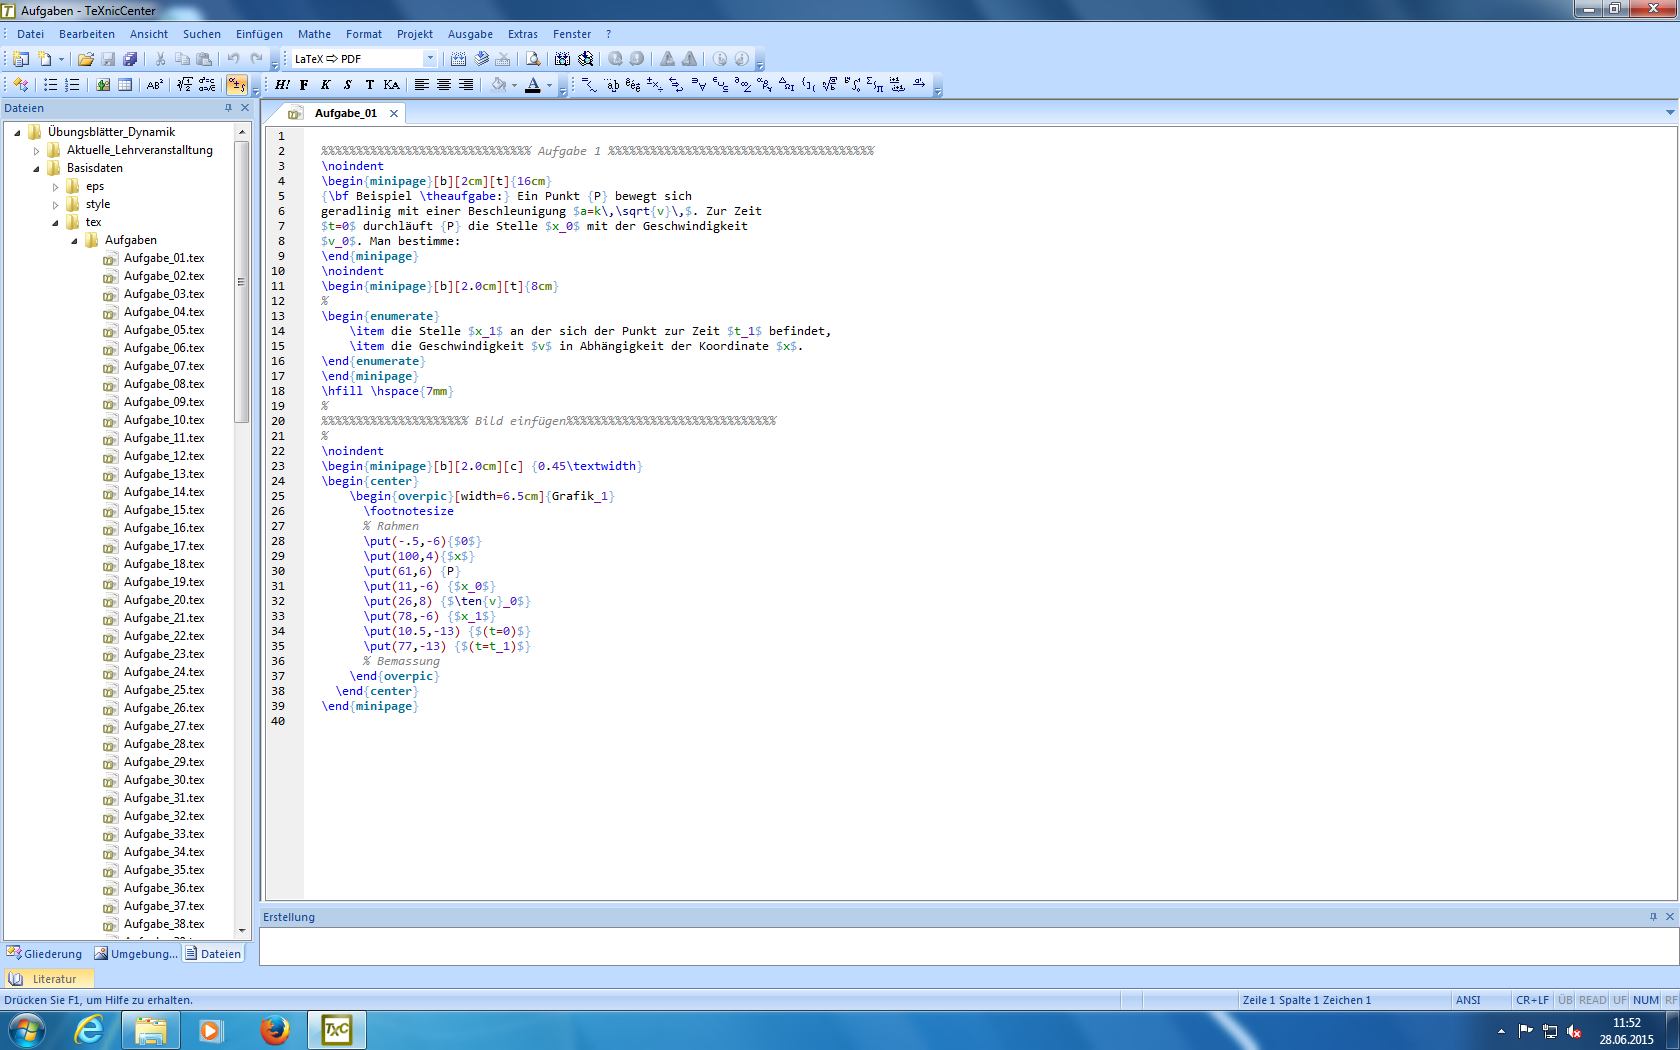
\includegraphics[width=\textwidth]{1_aufgabe01.png}
  \caption{Datei \twrite{Aufgabe\_01.tex}. Hier ist das eigentliche Beispiel
    definiert: Oben steht der Text zur Angabe, gefolgt von den Fragen. Darunter
    wird das Bild geladen und beschriftet.}
  \label{fig:aufgabe01}
\end{figure}

%EOF